%============================================================
% APPENDICE
%============================================================
\begin{appendices}

\section{Implementation Details}\label{app:implementation}

%%%%%%%%%%%%%% PARLARE dei dettagli implementativi, i.e. GPU usaste, versione di pytorch/python, etc

\subsection{Preprocessing Pipeline Details}\label{app:preprocessing}

This appendix provides the full mathematical formulation of the preprocessing pipeline summarized in Section~\ref{sec:experiments}.

\subsubsection{Binarization as an Auxiliary Mask}

Binarization is used exclusively to \emph{compute} crop coordinates and content masks. 
Concretely, each image is first converted to grayscale and, from it, an Otsu-thresholded binary version is derived and 
used only as a guide for locating text regions. Otsu's method determines the optimal threshold $t^*$ by maximizing inter-class variance:
\begin{equation}
t^* = \arg\max_t \sigma_B^2(t) = \arg\max_t \omega_0(t) \omega_1(t) [\mu_0(t) - \mu_1(t)]^2
\end{equation}
where $\omega_0(t)$ and $\omega_1(t)$ represent background and foreground class probabilities, and $\mu_0(t)$, $\mu_1(t)$ are their respective means. The resulting binary mask has text pixels set to 0 (black) and background to 255 (white), and is used downstream for: (i) detecting IAM guide lines, (ii) locating left-margin black columns and top/bottom black rows, and (iii) computing tight-crop bounding boxes. All crop coordinates derived from the binary mask are then applied to the corresponding grayscale image, which is what is actually cropped, resized, and written to the output dataset.

\subsubsection{Tight Cropping}
\label{app:tight-cropping}

To eliminate excessive whitespace while preserving text content, we compute tight crop coordinates using axial projections on the binary mask, and apply the resulting bounding box to the grayscale image. For a binary image $I$ of size $h \times w$, we invert it ($I_{\text{inv}} = 255 - I$) and compute row and column projections:
\begin{equation}
S_{\text{row}}(i) = \sum_{j=1}^{w} \mathbb{I}[I_{\text{inv}}(i,j) > 0], \quad S_{\text{col}}(j) = \sum_{i=1}^{h} \mathbb{I}[I_{\text{inv}}(i,j) > 0]
\end{equation}

Adaptive thresholds determine content-bearing rows and columns, based on a minimum ink-density ratio $\rho$:
\begin{equation}
\tau_{\text{row}} = \max(10, \lfloor \rho \cdot w \rfloor), \quad \tau_{\text{col}} = \max(10, \lfloor \rho \cdot h \rfloor)
\end{equation}
By default $\rho = 0.018$ (used for RIMES line processing); for IAM full-form images we use a slightly stricter $\rho = 0.02$ to compensate for residual guide-line artifacts left after region extraction.

The bounding box is defined by:
\begin{equation}
y_1 = \min\{i : S_{\text{row}}(i) > \tau_{\text{row}}\}, \quad y_2 = \max\{i : S_{\text{row}}(i) > \tau_{\text{row}}\}
\end{equation}
\begin{equation}
x_1 = \min\{j : S_{\text{col}}(j) > \tau_{\text{col}}\}, \quad x_2 = \max\{j : S_{\text{col}}(j) > \tau_{\text{col}}\}
\end{equation}

A 3-pixel internal trim, applied only along the row axis, removes residual guide lines: $y_1 \leftarrow \min(y_1+3,\, y_2-1)$ and $y_2 \leftarrow \max(y_2-3,\, y_1+1)$, while $x_1, x_2$ are left untouched. This is followed by 5-pixel padding on \emph{all four} sides to prevent text from touching borders. The resulting coordinates $(y_1, y_2, x_1, x_2)$ are then used to crop the grayscale image, not the binary mask.

\subsubsection{Aspect-Preserving Resize}

Images are normalized to 448×448 pixels by first centering them in a square canvas of side $s = \max(h, w)$ with offsets:
\begin{equation}
\text{offset}_y = \lfloor (s - h) / 2 \rfloor, \quad \text{offset}_x = \lfloor (s - w) / 2 \rfloor
\end{equation}
The canvas is then resized to 448×448 using area interpolation, preserving the original aspect ratio without distortion.

\subsubsection{IAM Dataset Preprocessing}

IAM forms contain pre-printed guide lines that must be removed. We detect horizontal lines using morphological opening (erosion followed by dilation, 2 iterations) with a kernel of width $k_w = \max(30, \lfloor w/15 \rfloor)$:
\begin{equation}
\text{Opening}(I, K) = \text{Dilate}(\text{Erode}(I, K), K)
\end{equation}

Valid lines satisfy: $w_c > 0.3w$, $h_c < 20$, and area $> 100$ pixels. Detected lines are sorted top-to-bottom and the handwritten region is selected according to how many valid lines are found:

\begin{itemize}
\item \textbf{Three or more lines detected:} the region is extracted between the second and third detected lines,
\begin{equation}
y_{\text{start}} = y_{\text{bottom}}^{(2)} + 8, \quad y_{\text{end}} = y_{\text{top}}^{(3)} - 8
\end{equation}

\item \textbf{Exactly two lines detected:} the region is extracted between them,
\begin{equation}
y_{\text{start}} = y_{\text{bottom}}^{(1)} + 8, \quad y_{\text{end}} = y_{\text{top}}^{(2)} - 8
\end{equation}

\item \textbf{Fewer than two lines detected:} a secondary detection pass estimates guide-line positions from a smoothed row-density profile. The row-wise ink density is smoothed with a uniform filter (window size 5), and rows exceeding the 95th percentile of the smoothed profile are grouped into contiguous line segments (gap tolerance of 5 pixels). If this secondary pass yields three or more segments, or exactly two, the same rules above are re-applied to the segments; otherwise the pipeline falls back to a fixed region.

\item \textbf{Fallback:} if no reliable lines are found by either pass,
\begin{equation}
y_{\text{start}} = \lfloor 0.22h \rfloor, \quad y_{\text{end}} = \lfloor 0.85h \rfloor
\end{equation}
\end{itemize}

As a final safeguard, if the extracted region is empty or smaller than $30 \times 50$ pixels (height $\times$ width), extraction reverts to the fixed fallback region above. Guide-line detection and region selection are performed on the binary mask, but the corresponding rows are extracted from \emph{both} the grayscale and binary versions of the image, keeping them spatially aligned for the subsequent steps. After region extraction, black column removal (removing columns with $>50\%$ black pixels from the left margin, computed on the binary region) and tight cropping (coordinates computed on the binary region with $\rho = 0.02$, Appendix~\ref{app:tight-cropping}) are applied to the grayscale region before final resizing. The binary region itself is discarded after this point and never saved. Figure~\ref{fig:iam-preprocessing} illustrates this pipeline end to end, from the original grayscale form to the final cropped and resized image.

Two additional sanity checks guard against degenerate cases. First, immediately after $y_{\text{start}}$ and $y_{\text{end}}$ are determined by any of the branches above, if $y_{\text{start}} \geq y_{\text{end}}$ (an invalid, empty, or inverted range) the pipeline discards that estimate and reverts directly to the fixed fallback $[0.22h, 0.85h]$. Second, whichever values of $y_{\text{start}}, y_{\text{end}}$ are ultimately used are clipped to the valid image range, $y_{\text{start}} \leftarrow \max(0, y_{\text{start}})$ and $y_{\text{end}} \leftarrow \min(h, y_{\text{end}})$, before the region is sliced from the image. This clipping is independent of, and precedes, the minimum-size safeguard described above.

\begin{figure}[h]
\centering
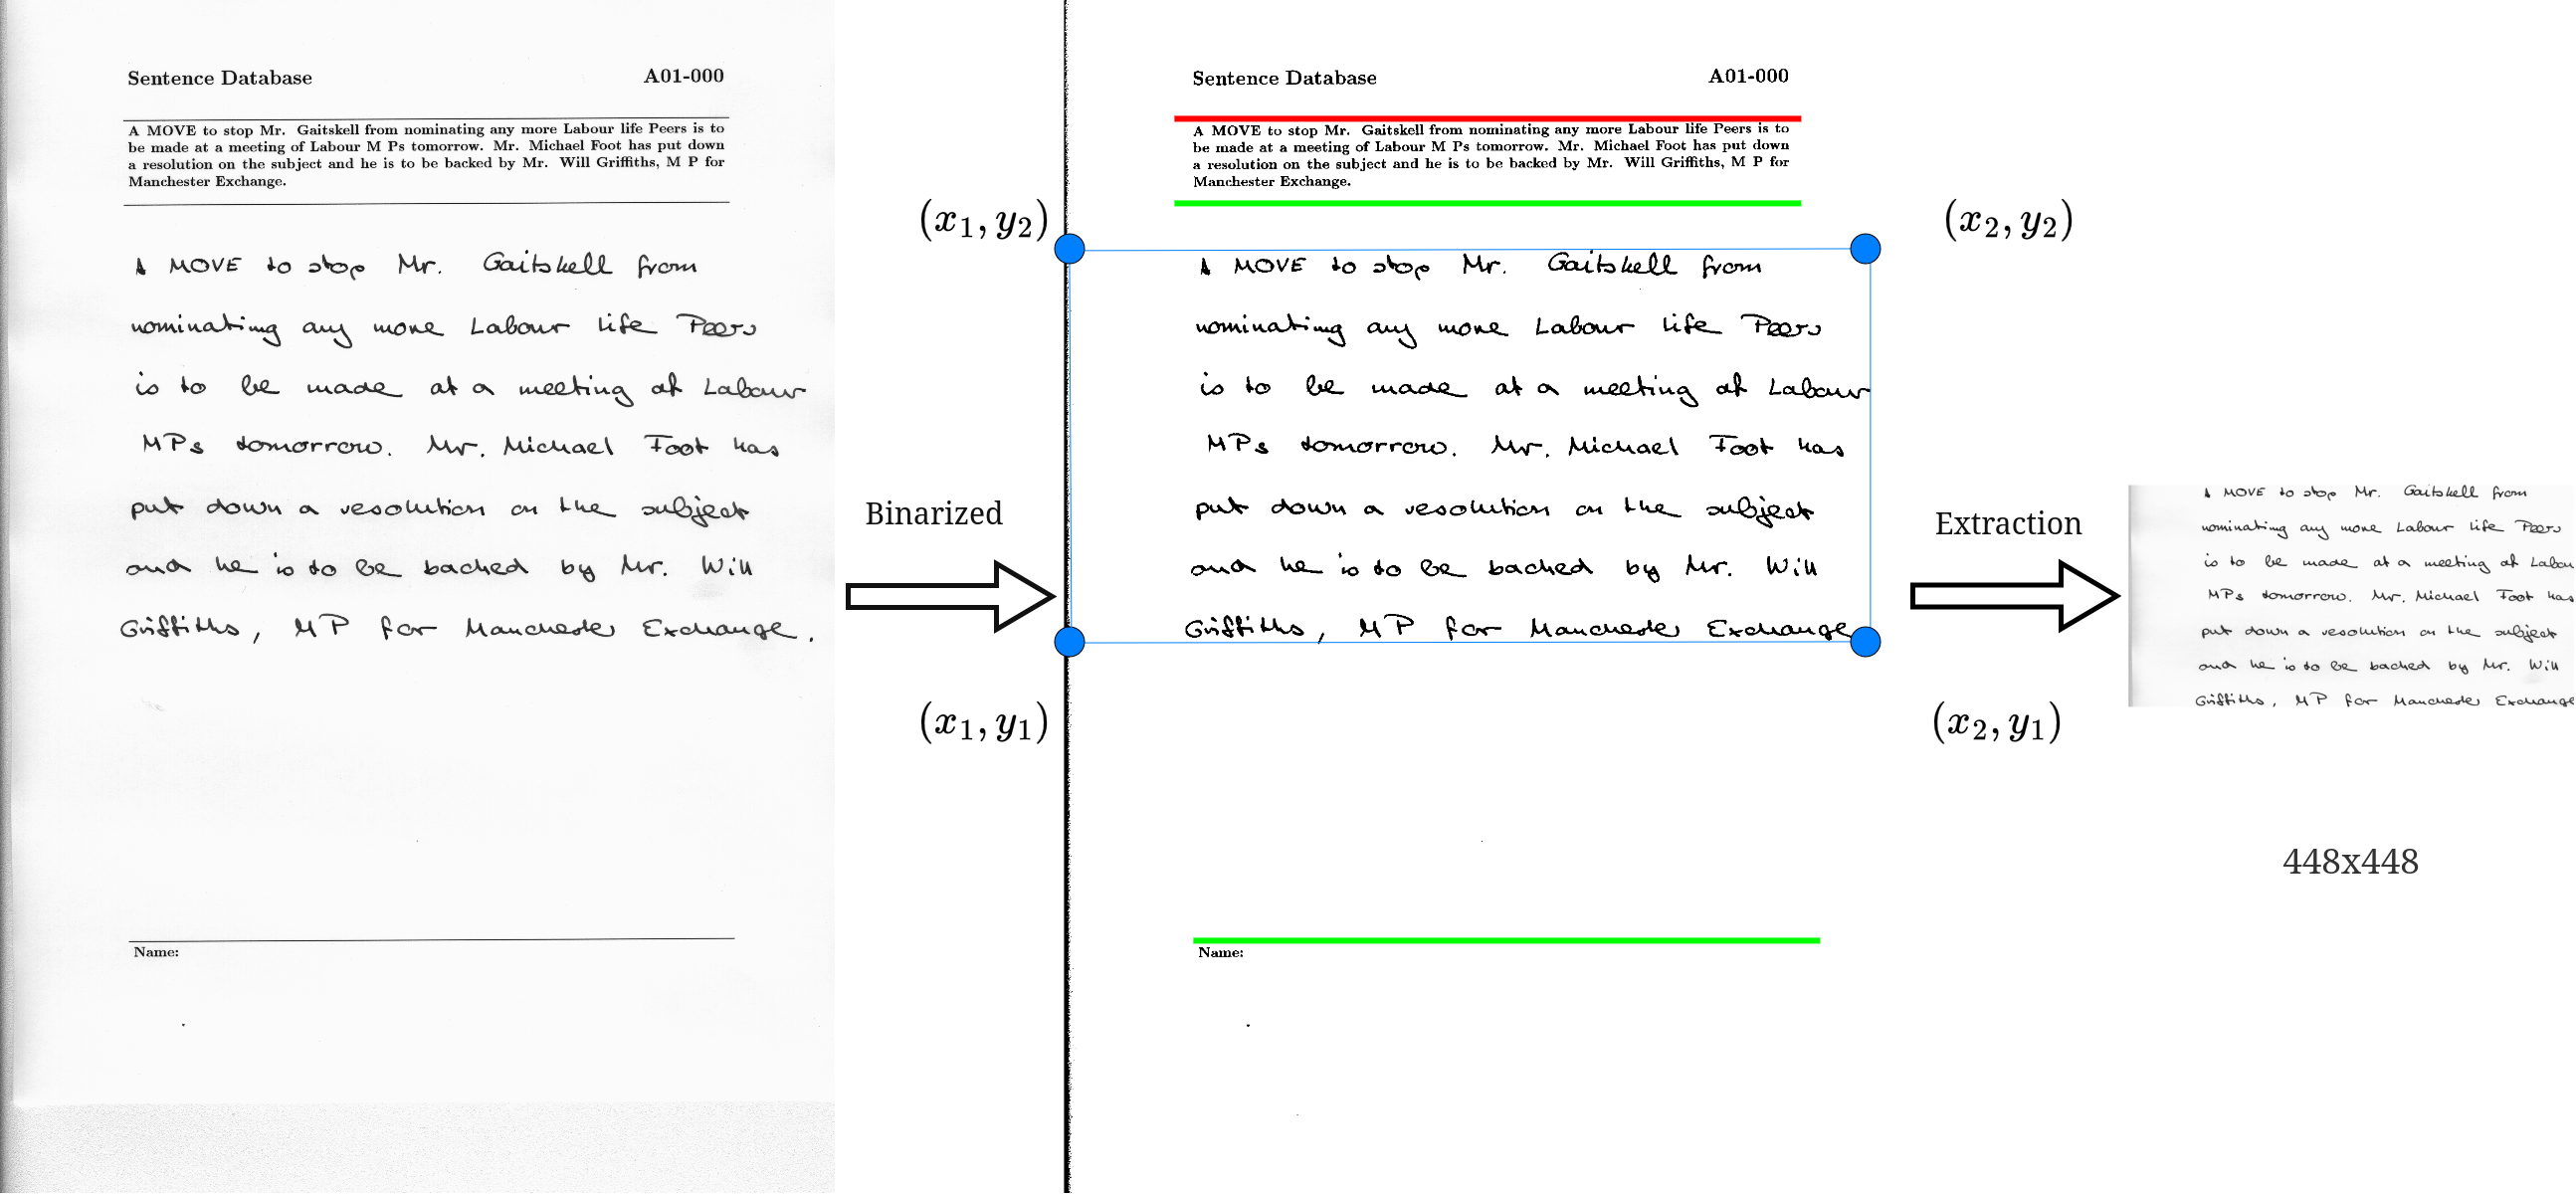
\includegraphics[width=0.9\linewidth]{images/iam-preprocessing.png}
\caption{Preprocessing of an IAM form: the grayscale image (left) is binarized (center) to detect guide lines (red/green, detected by erosion/dilation) and the handwritten text region (blue box); this region is then extracted from the original grayscale image, cropped, and resized to 448×448 pixels (right).}
\label{fig:iam-preprocessing}
\end{figure}

\subsubsection{RIMES Dataset Preprocessing}
\label{app:rimes-preprocessing}

RIMES consists of individual text lines that are processed and stacked vertically to form 448×448 batches. Each line is first converted to grayscale, and an auxiliary Otsu binary mask is derived from it (as described above) purely to guide cropping; only the grayscale line is cropped, resized, and eventually stacked into the output batch. Each line undergoes:

\begin{enumerate}
\item \textbf{Vertical trim:} Removal of rows with $>50\%$ black pixels from top and bottom, computed on the binary mask and applied identically to both the mask and the grayscale line
\item \textbf{Tight cropping:} Bounding-box coordinates computed on the binary mask via the projection-based algorithm ($\rho = 0.018$, Appendix~\ref{app:tight-cropping}), applied to crop the grayscale line
\item \textbf{Height normalization:} For each writer, the minimum observed line height across all their (cropped) lines is computed and clamped to the range $[20, 32]$ pixels, $h_{\min} = \text{clip}(\min_l h_l,\ 20,\ 32)$. All lines from that writer are then resized to height $h_{\min}$, preserving aspect ratio:
\begin{equation}
w' = \lfloor w \cdot h_{\min} / h \rfloor
\end{equation}
If the resulting width $w'$ exceeds the target canvas width (448 px), the line is instead scaled down so that $w' = 448$ and $h' = \lfloor h \cdot 448/w \rfloor \le h_{\min}$. Each resized line is placed on a fixed-size $h_{\min} \times 448$ white canvas, left-aligned and vertically centered with offset $\lfloor (h_{\min} - h')/2 \rfloor$.
\item \textbf{Batching:} Height-normalized lines are vertically stacked into groups of $N_{\text{batch}} = \lfloor 448 / 32 \rfloor - 9 = 5$ lines per batch, producing $448\times448$ canvases per writer. The last batch for a writer is padded with white space if fewer than $N_{\text{batch}}$ lines remain. Figure~\ref{fig:rimes-preprocessing} illustrates this pipeline, from original lines to tight-cropped lines and their grouping into stacked $448\times448$ batches.
\end{enumerate}

Lines exceeding 896 pixels in width (twice the target size) are split at the midpoint before height normalization, to prevent excessive aspect ratio distortion. This produces uniform-height stacked representations suitable for Siamese network training. Note that with $N_{\text{batch}} = 5$ lines of at most 32 px height each, a batch occupies at most 160 of the 448 available vertical pixels; the remaining space is white padding.

\begin{figure}[h]
\centering
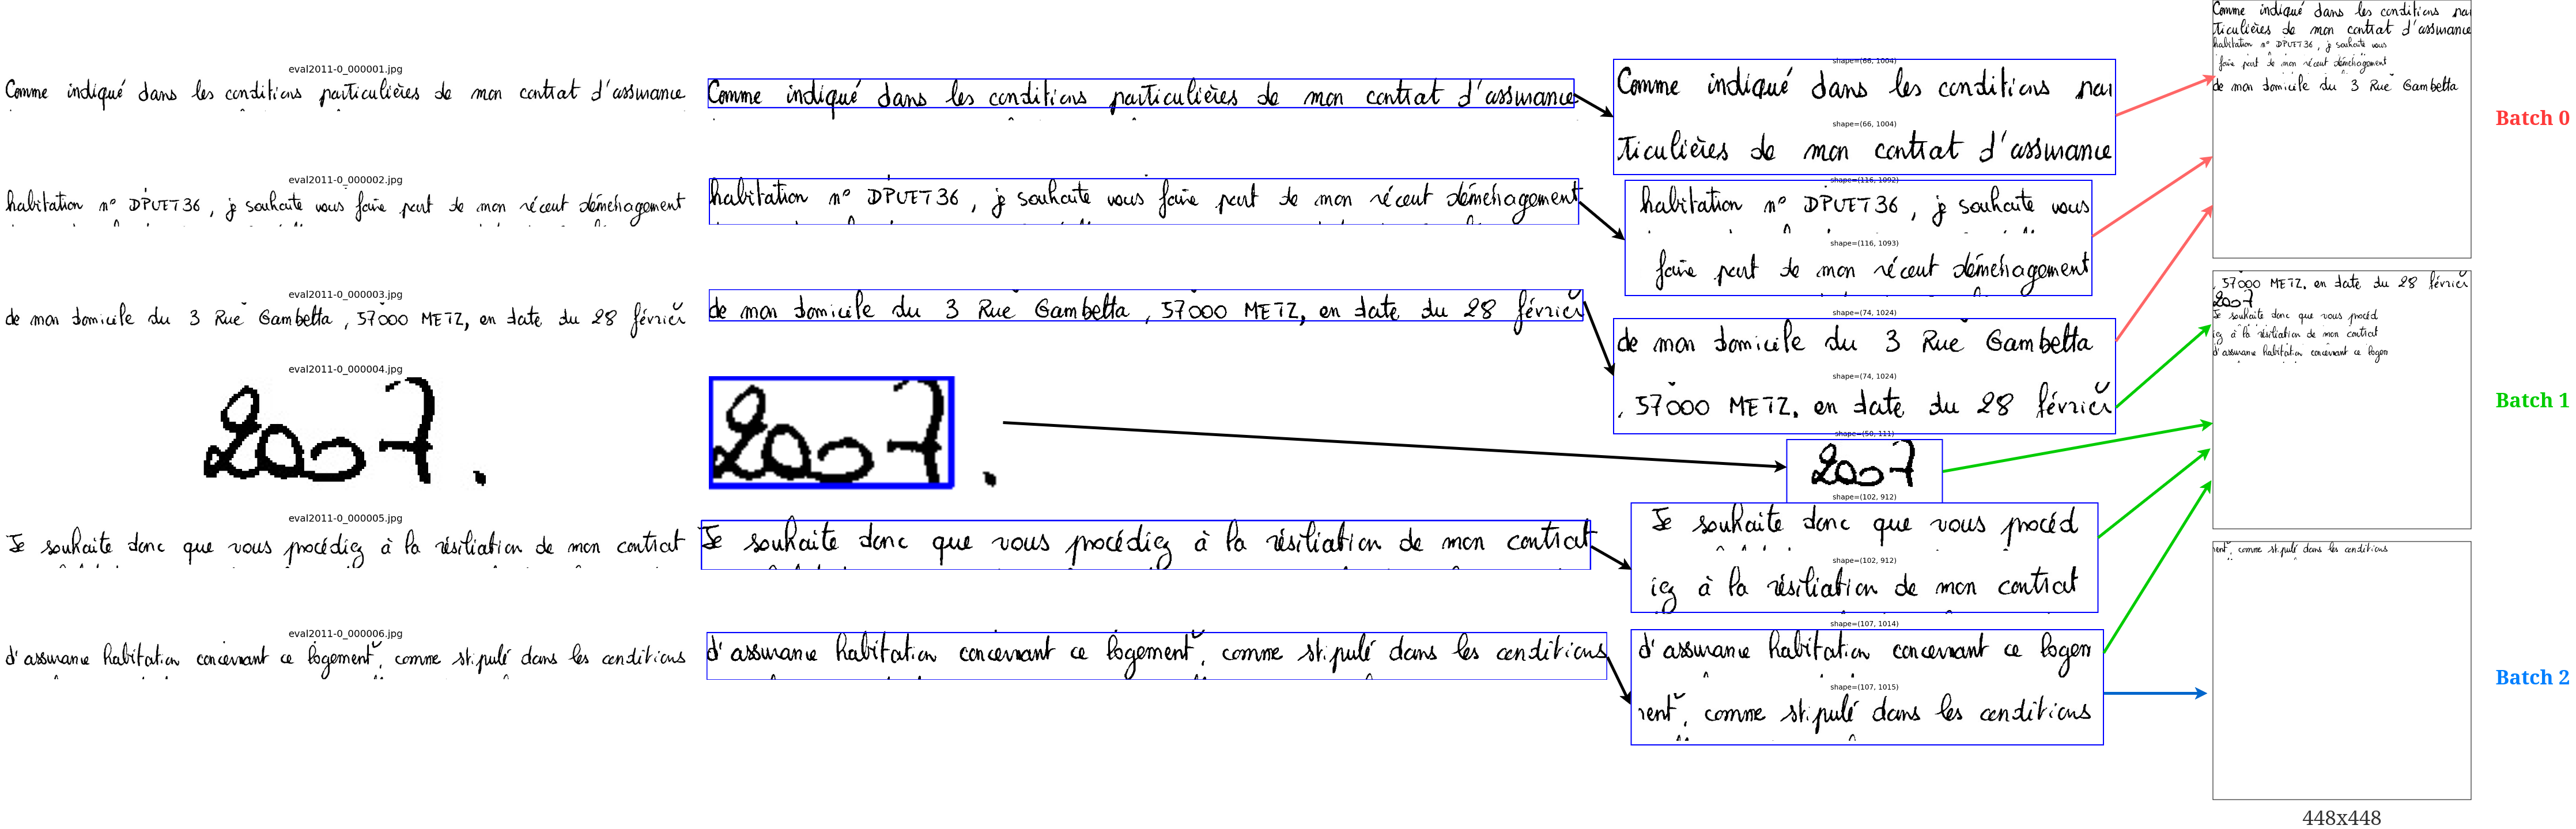
\includegraphics[width=1.0\linewidth]{images/rimes-preprocessing.png}
\caption{Preprocessing of RIMES text lines (for a given author). Each original line (left, e.g. \texttt{eval2011-0\_000001.jpg}) is binarized via Otsu thresholding and tight-cropped (blue bounding boxes, center) using the projection-based algorithm; the corresponding grayscale crop is then extracted (right of center). Cropped lines belonging to the same writer are grouped (colored arrows) and vertically stacked into fixed-size $448\times448$ canvases (right), with unused space padded in white.}
\label{fig:rimes-preprocessing}
\end{figure}

\subsection{Dataset Statistics: Distribution Figures}\label{app:dataset-stats-figures}

Figure~\ref{fig:dataset-distribution} shows the per-author image count distributions for both datasets after preprocessing, complementing the summary statistics of Table~\ref{tab:dataset-stats}. The IAM histogram (top) is dominated by a large spike at 1--2 images per author, with a long, sparse tail extending up to the outlier author with 59 images. The RIMES histogram is comparatively broader and shifted toward higher counts, peaking around 3 batches per author and extending up to 10, reflecting a more even but still right-skewed spread. The boxplot comparison (bottom) further highlights this asymmetry: IAM's interquartile range is narrow and close to zero, with the extreme outlier and long upper whisker revealing a much heavier tail, while RIMES shows a wider, more centrally distributed spread with a shorter relative tail.

\begin{figure}[h]
\centering
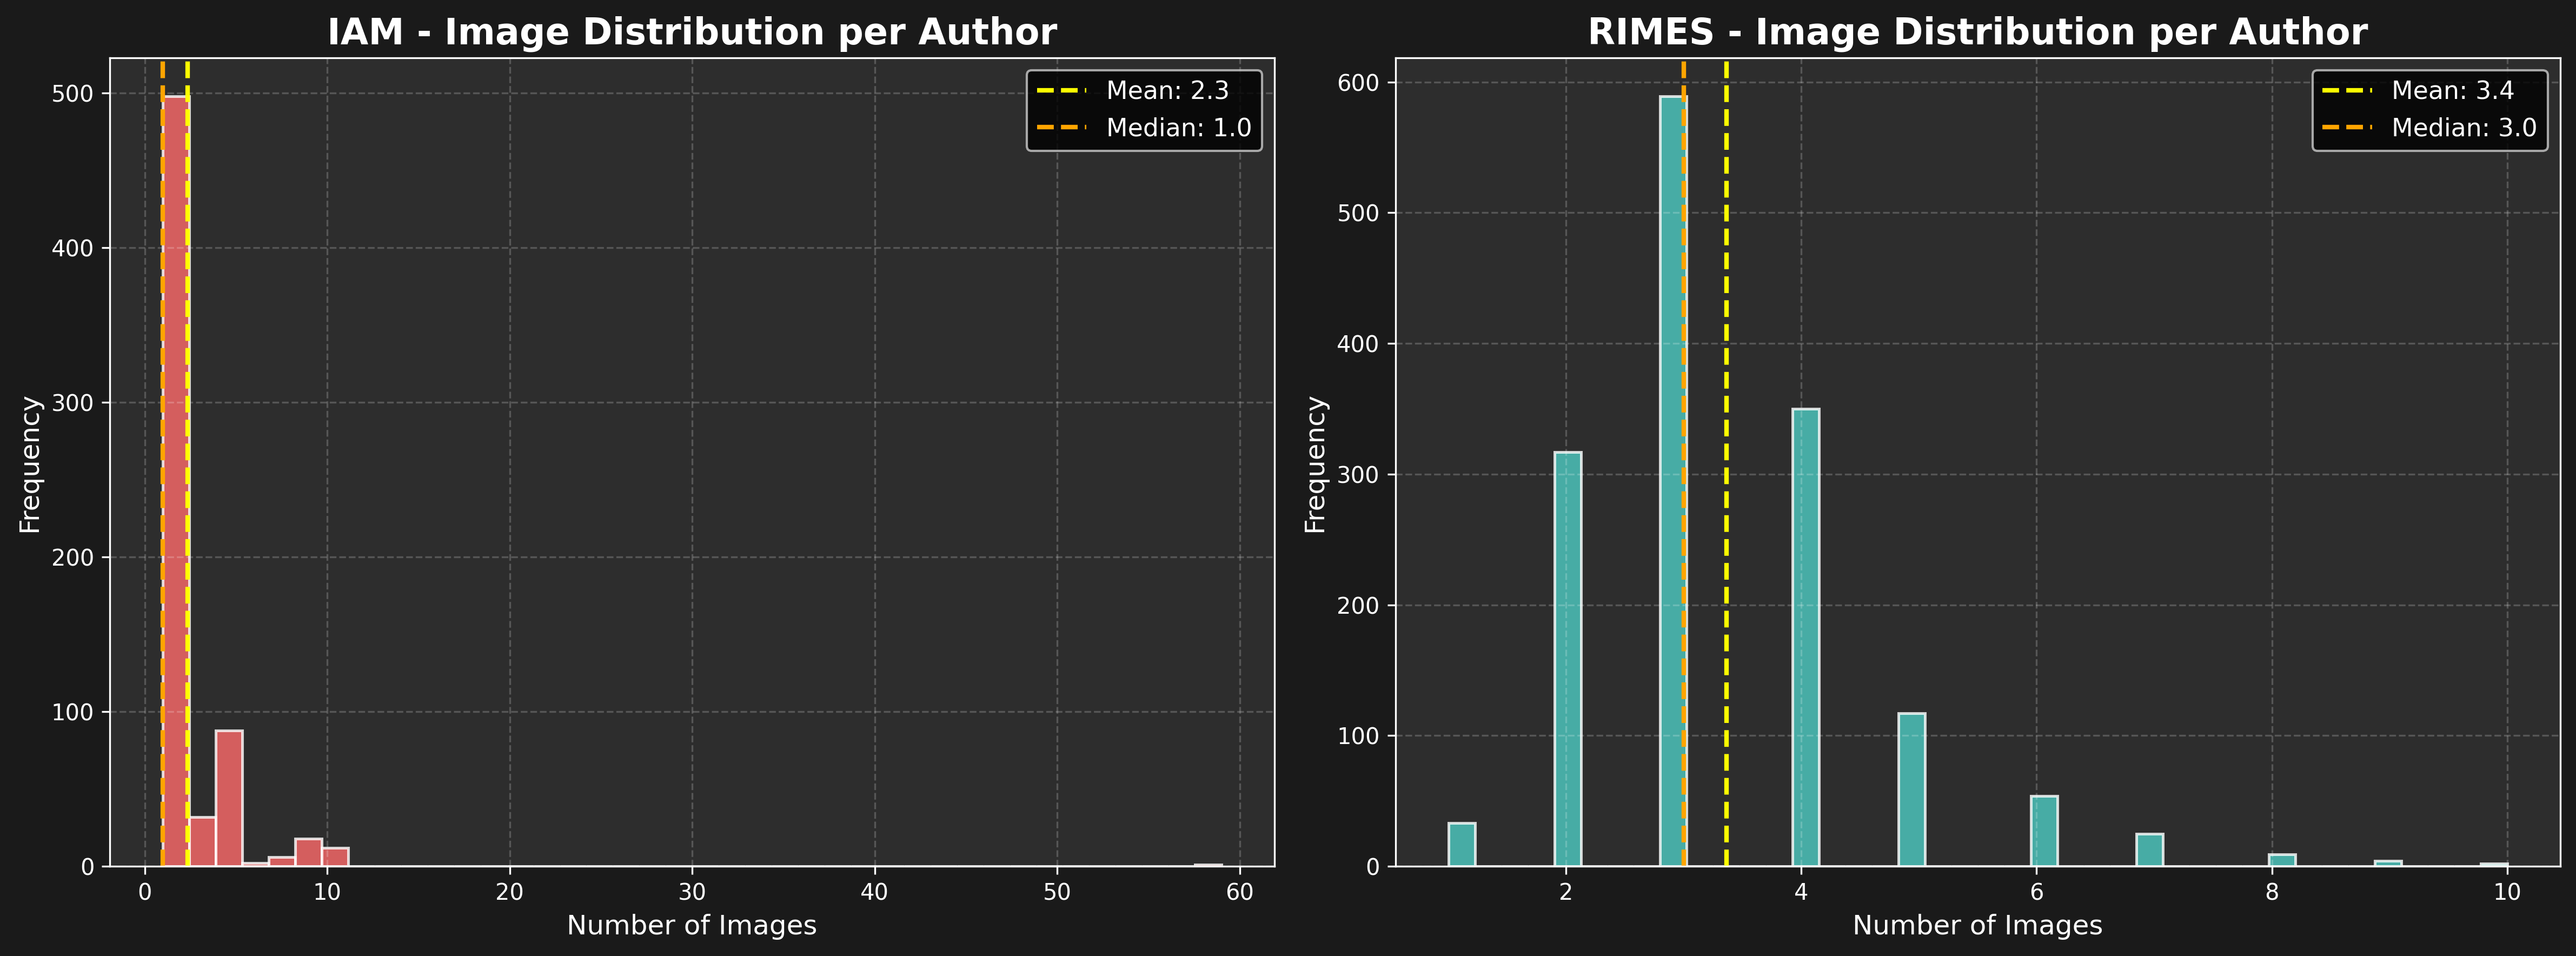
\includegraphics[width=0.65\linewidth]{images/distribution_images.png}
\\[0.5em]
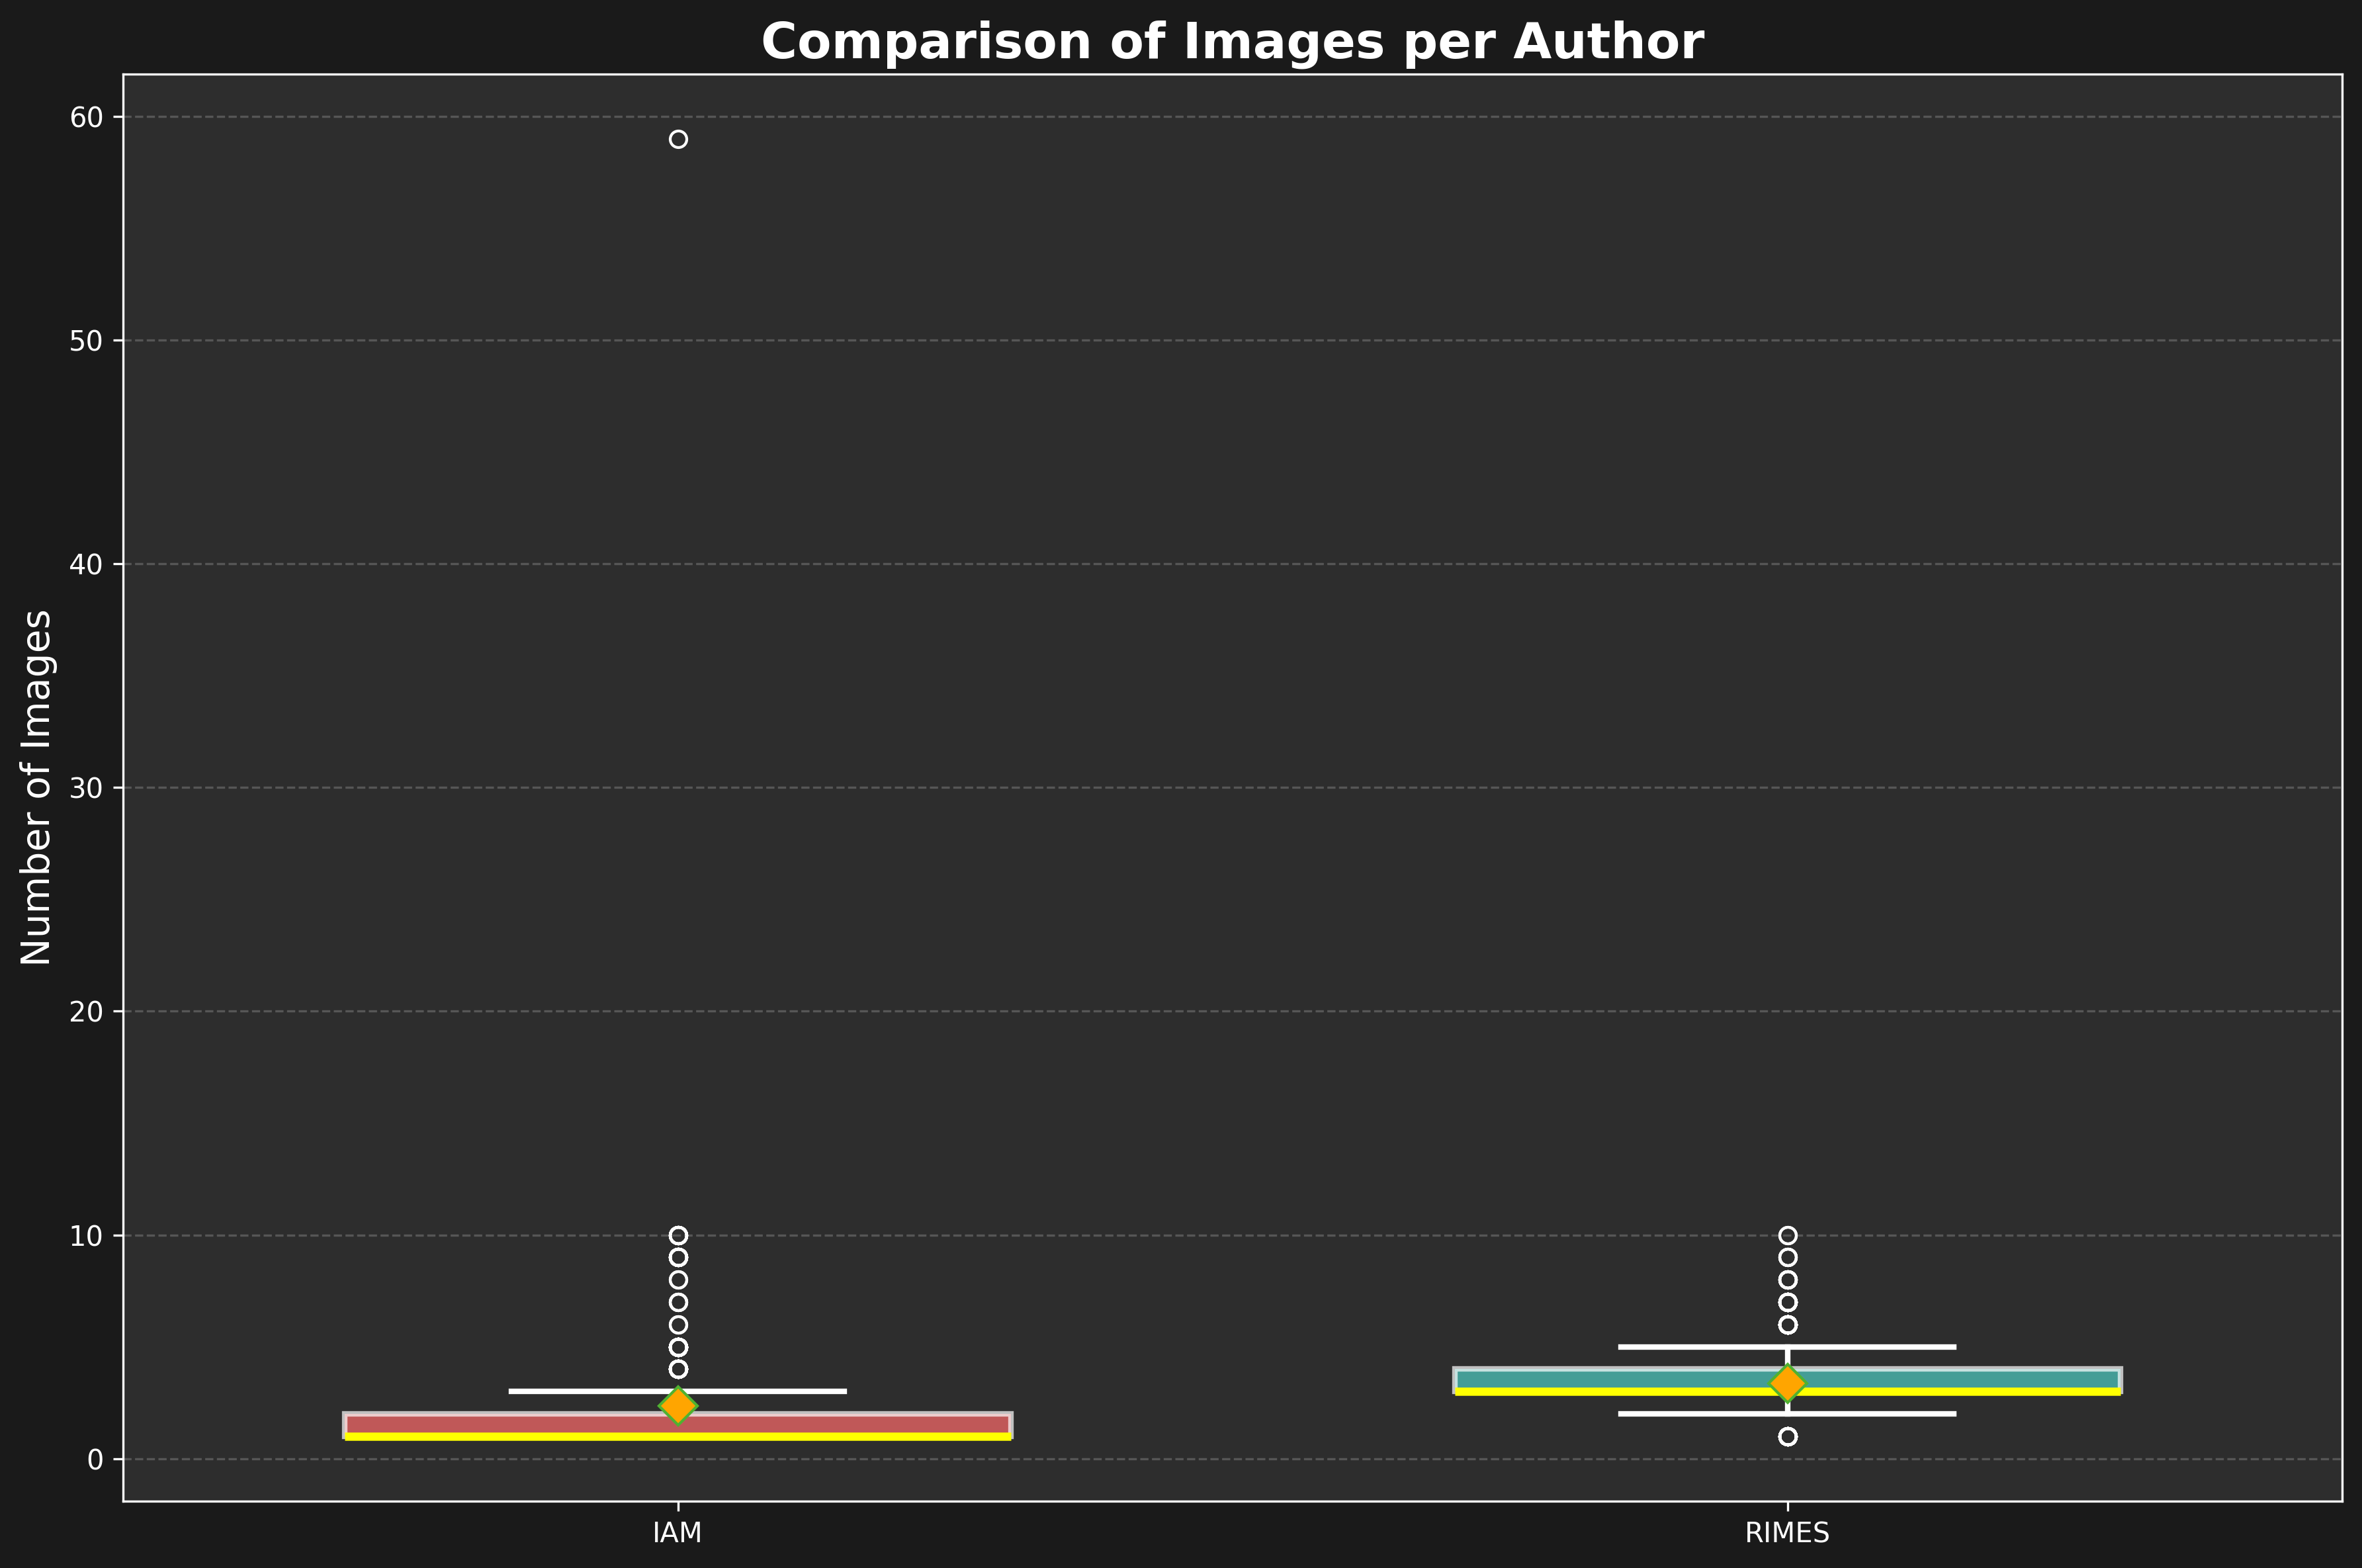
\includegraphics[width=0.7\linewidth]{images/boxplot_comparison.png}
\caption{Distribution of images per author for the preprocessed IAM and RIMES datasets. \textbf{Top:} per-dataset histograms with mean (yellow) and median (orange) overlaid, showing the strong right skew of IAM compared to the broader, more centrally distributed RIMES spread. \textbf{Bottom:} side-by-side boxplot comparison, highlighting the extreme outlier author in IAM (59 images) against the wider but shorter-tailed RIMES distribution (max 10 images).}
\label{fig:dataset-distribution}
\end{figure}

\subsection{Hyperparameter Configuration}\label{app:hyperparams}

Table~\ref{tab:hyperparams-appendix} summarizes the hyperparameter configuration used across the 72-model sweep, 
including values already discussed in the main text (Section~\ref{sec:experiments}) 
and additional training-setup details not otherwise reported, such as maximum epochs, 
embedding dimension, and data-loading workers. Loss-specific margins follow Section~\ref{sec:methodology}: 
$m=1.0$ for Contrastive and $m=0.5$ for Triplet.

\begin{table}[htbp]
\centering
\caption{Hyperparameter configuration shared across the 72 model configurations. Loss-specific settings are indicated where applicable.}
\label{tab:hyperparams-appendix}
\begin{tabular}{ll}
\hline
\textbf{Hyperparameter} & \textbf{Configuration} \\
\hline
Batch size & 16 \\
Maximum epochs & 50 \\
Early stopping & Patience = 5 \\
Image size & $448 \times 448$ pixels \\
Embedding dimension & 32 \\
Margin & 1.0 (Contrastive), 0.5 (Triplet) \\
Positive ratio & 0.5 \\
Dropout & 0.2 \\
Frozen encoder layers & 3 \\
Negative resampling & Every epoch (all losses) \\
Data-loading workers & 4 \\
\hline
\end{tabular}
\end{table}

\subsection{Training Dynamics}\label{app:training-curves}

Figure~\ref{fig:training_curves} reports training and validation loss curves for the ResNet-18 
backbone across all 12 loss$\times$split combinations. Across nearly all configurations, 
training loss decreases monotonically, consistent with stable optimization; however, 
validation-loss behavior differs substantially by loss function and split. Under BCE, 
validation loss tracks training loss relatively closely on the same-dataset splits 
(IAM$\to$IAM, RIMES$\to$RIMES), while the cross-dataset splits show an early divergence between 
the two curves (e.g., IAM$\to$RIMES), consistent with the same-vs-cross-dataset generalization 
gap discussed in Section~\ref{sec:cross-dataset}. Under Contrastive and, more markedly, 
under Triplet Loss, validation loss is considerably noisier and frequently non-monotonic, 
with pronounced oscillations and, in several cases (e.g., Triplet on IAM$\to$IAM and IAM$\to$RIMES), 
no clear downward trend despite steadily decreasing training loss -- indicative of a widening 
train--validation gap rather than smooth joint convergence. Training run lengths also vary 
considerably across configurations, from as few as 6 epochs (Triplet, RIMES$\to$RIMES) to 
over 40 (BCE, IAM$\to$IAM), reflecting the early-stopping criterion (patience 5, Appendix~\ref{app:hyperparams}) 
being triggered at different points depending on the stability of the validation signal for each configuration.

\begin{figure}[htbp]
  \centering
  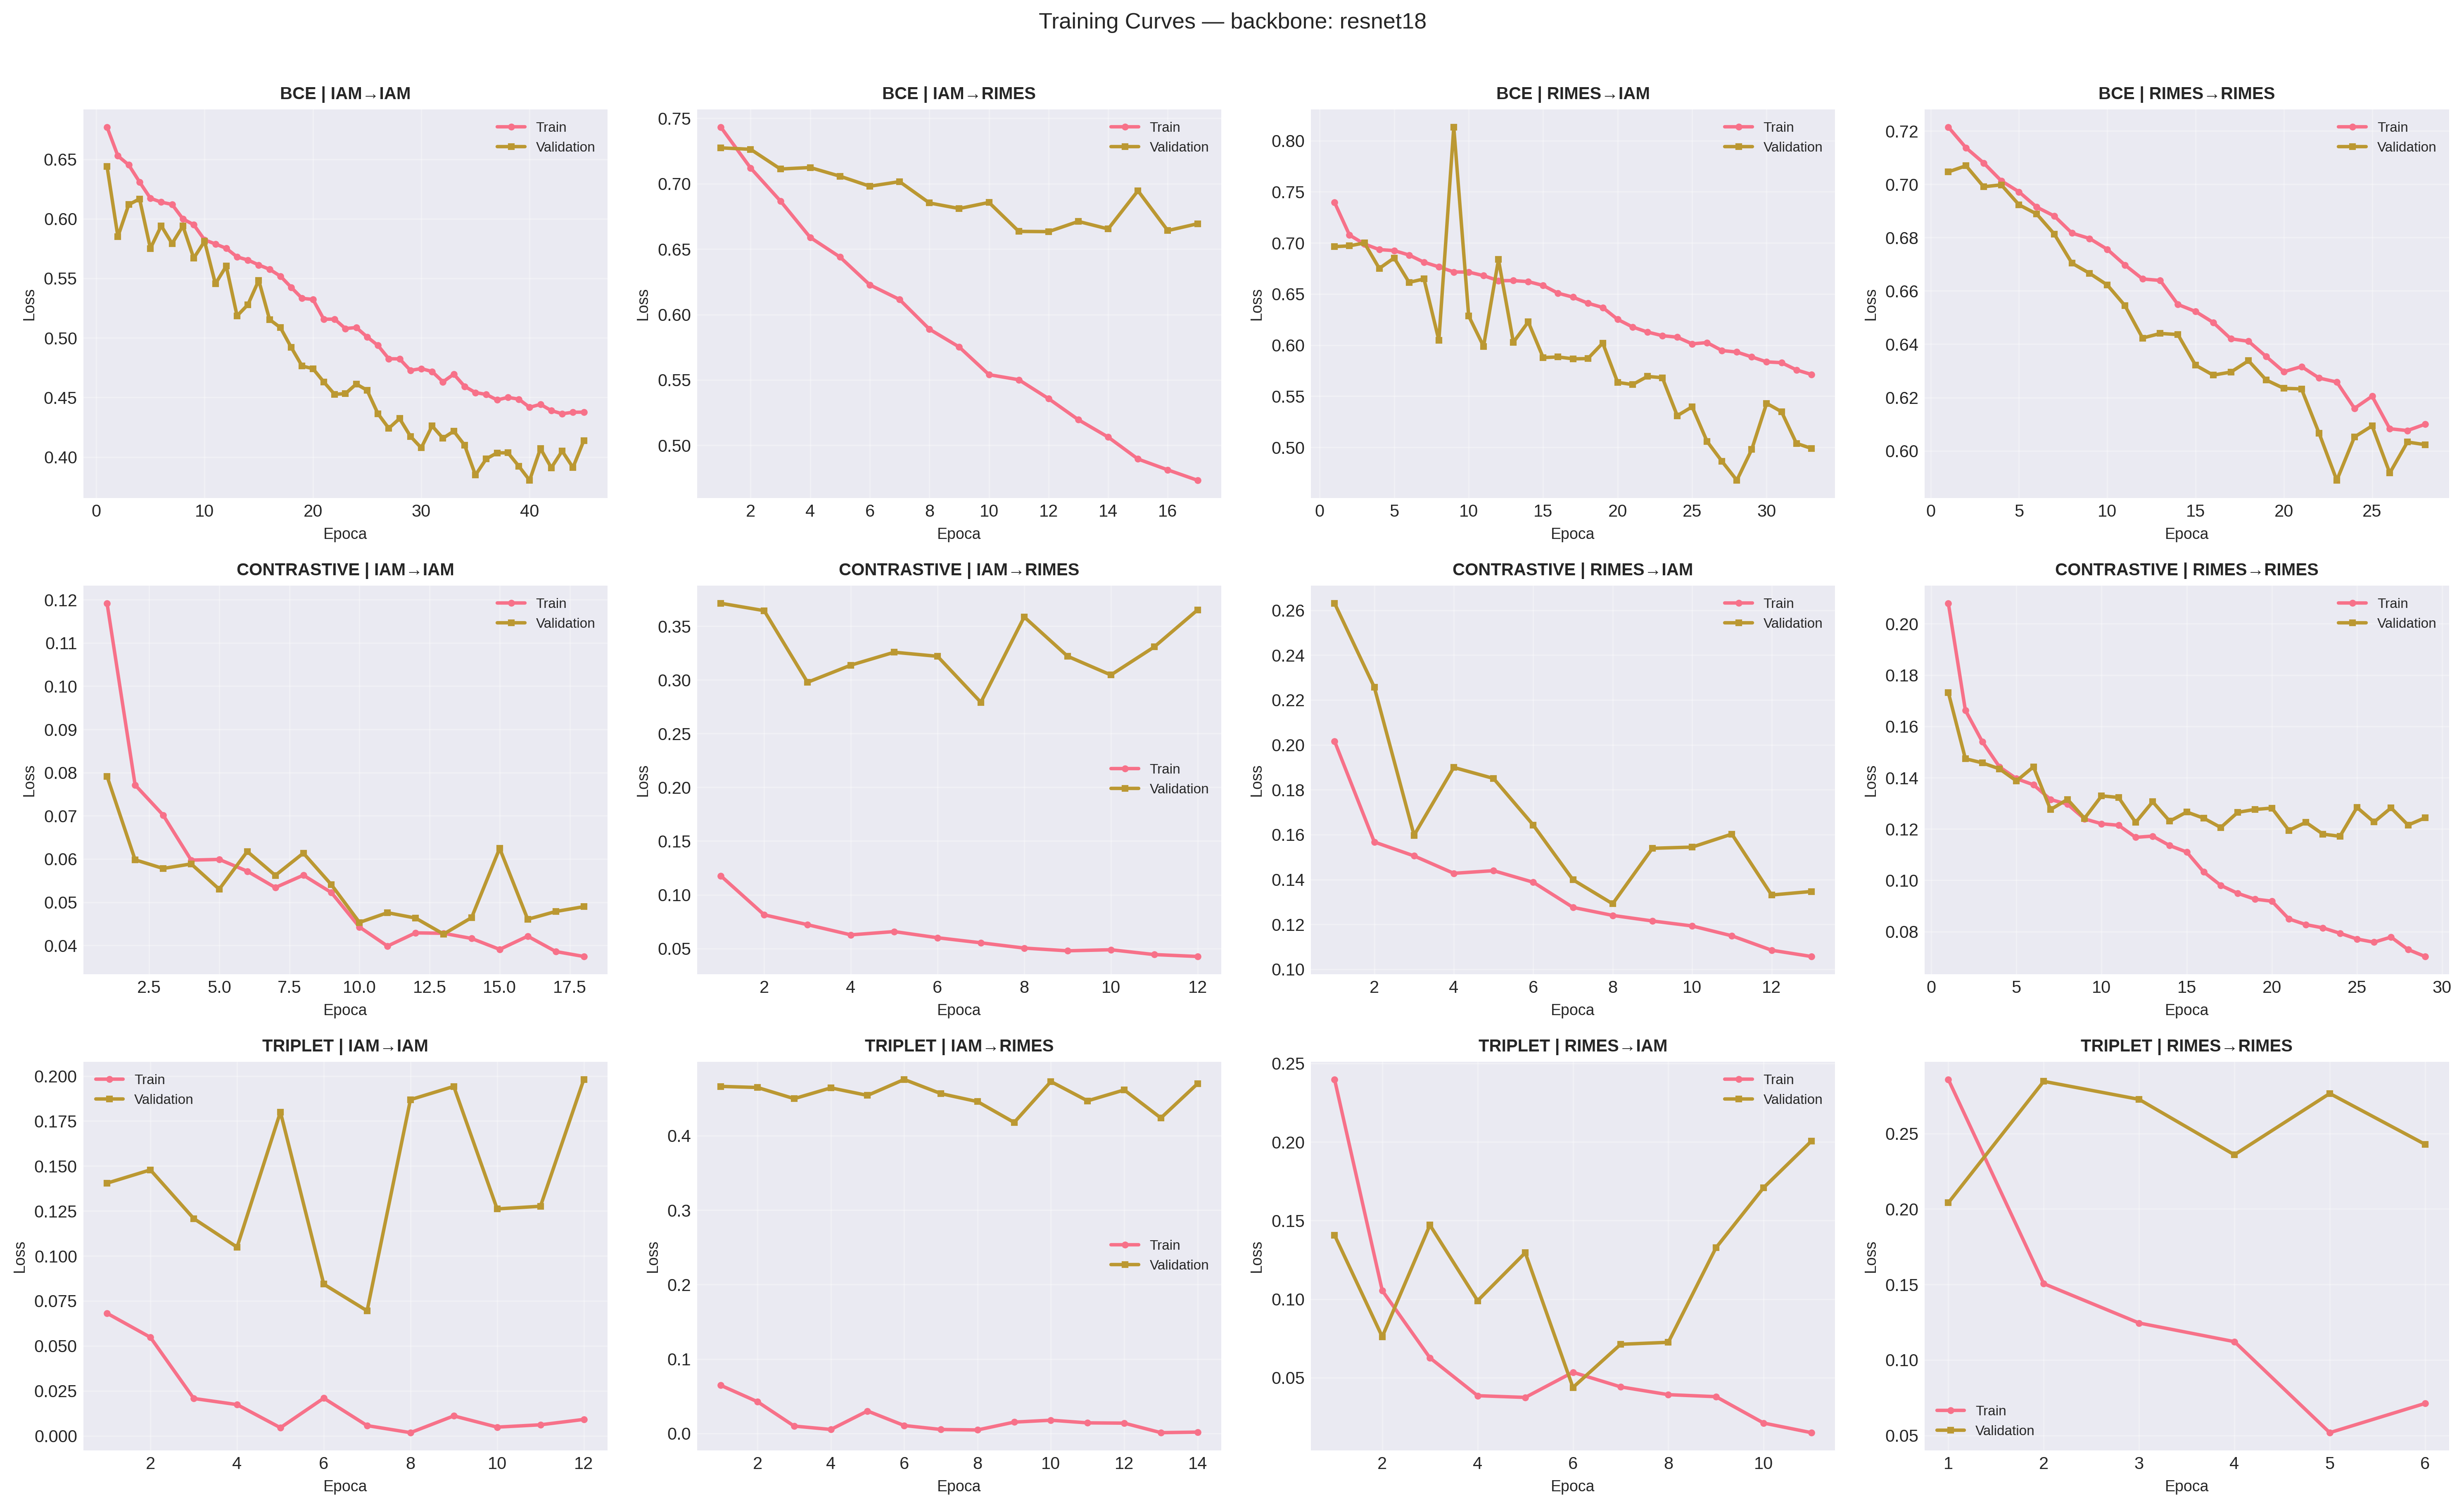
\includegraphics[width=\textwidth]{images/training_history_resnet18.png}
  \caption{Training and validation loss curves, ResNet-18, all 12 loss$\times$split combinations.}
  \label{fig:training_curves}
\end{figure}

\end{appendices}